\documentclass[lang=cn,newtx,10pt,scheme=chinese]{elegantbook}


\title{物理必修三整理}

\date{\today}

\setcounter{tocdepth}{3}

\cover{cover.jpg}

% 本文档命令
\usepackage{array}
\newcommand{\ccr}[1]{\makecell{{\color{#1}\rule{1cm}{1cm}}}}

% 修改标题页的橙色带
\definecolor{customcolor}{RGB}{32,178,170}
\colorlet{coverlinecolor}{customcolor}
\usepackage{cprotect}

\addbibresource[location=local]{reference.bib} % 参考文献,不要删除

\begin{document}

\maketitle
\frontmatter

\tableofcontents

\mainmatter

\setcounter{chapter}{8}
\chapter{静电场及其应用}
\section{电荷}
\subsection{电荷}

\begin{definition}
    电荷的多少叫做\textbf{电荷量(electric quantity)},用 $Q$ 或者 $q$ 表示,单位为 \textbf{库伦 (coulomb)},简称  \textbf{库},符号为 $C$。
\end{definition}

\subsection{静电感应}

带电体靠近导体,由于电荷间的相互吸引或者排斥,导体中的自由电荷会趋向或者远离带点体。这种现象叫做\textbf{静电感应(electrostatic induction)}。

\subsection{电荷守恒定律}

\begin{theorem}
  大量实验事实表明,电荷既不会创生,也不会消灭,只能从一个物体转移到另一个物体,或者从物体的一部分转移到另一个部分;在转移的过程中,电荷总量保持不变。这个结论叫做\textbf{电荷守恒定律(law of conservation of charge)}。
\end{theorem}

\subsection{元电荷}

电子带的电量是目前发现的最小电荷量,称为 \textbf{元电荷(elementary charge)},用 $e$ 表示。密立根的油滴实验测得元电荷的电量,经过后人的补测得到公认的值为:

$$
e = 1.602176634\times 10^{-19} \text{C}
$$

计算中为了方便常取 $\displaystyle e=1.60\times10^{-19}\text{C}$

比荷:电荷量 $q$ 和质量 $m$ 的比值称为\textbf{比荷(specific charge)},用 $\displaystyle \frac{q}{m}$ 表示。电子的比荷为:

$$
\frac{e}{m_e} = 1.76\times 10^{11} \text{C/kg}
$$

\section{库伦定律}

\subsection{电荷之间的作用力}

真空中两个静止的点电荷之间的相互作用力与其电荷量的乘积成正比,距离的平方成反比,这个规律被称为\textbf{库伦定律(Coulomb's law)},力称为静电力或者库仑力。

库伦实验表明:

$$
F = k\frac{q_1q_2}{r^2}
$$

\begin{itemize}
  \item $k=9.0 \times 10^9 \text{N} \cdot \text{m}^2 / \text{C}^2$ 称为静电力常量
  \item 库伦力为矢量,遵循矢量的叠加原理,并且当 $q_1$ 和 $q_2$ 异号时,库伦力为吸引力,同号时为斥力。
  \item 库伦力的方向沿着两点电荷连线。
\end{itemize}

\section{电场和电场强度}

\subsection{电场}

法拉第提出的\textbf{电场(electric field)}概念\footnote{Faraday 提出的是力线的概念,电场的概念是 Maxwell 等人完善的},认为电场中粒子收到的力的作用是由电场给与的。

\begin{note}
  在本章中只考虑静止电荷产生的\textbf{静电场(electrostatic field)}
\end{note}

\subsection{电场强度}

试探电荷:在电场中放置一个很小的正电荷,称为\textbf{试探电荷(test charge)}。这个电荷的大小足够小,以至于它在电场中不会改变电场的分布。激发带你常的带电梯所带的电荷叫做\textbf{场源电荷},或者\textbf{源电荷}。

\begin{definition}
  实验表明,电场中试探电荷受到的力与其电荷大小无关。这个比值反映了电场在各点的性质,叫做\textbf{电场强度(electric field strength)},用 $E$ 表示。定义为:

  $$
  E = \frac{F}{q}
  $$

  电场的强度的单位为 $\text{N}/\text{C}$,对于正电荷,其受到的力与电场强度的方向相同;对于负电荷,其受到的力与电场强度的方向相反。
\end{definition}

\subsection{点电荷德电场,电场强度的叠加}

\begin{theorem}
  点电荷 $Q$ 在空间某点产生的电场强度为:

  $$
  E = k\frac{Q}{r^2}
  $$

  其中 $k=9.0 \times 10^9 \text{N} \cdot \text{m}^2 / \text{C}^2$,$r$ 为点电荷到该点的距离。

  如果空间中有多个点电荷,则它们在某点产生的电场强度是各个点电荷在该点产生的电场强度的矢量和。
  即:
  $$
  \vec{E} = \sum_{i=1}^{n} \vec{E_i}
  $$
  其中 $\vec{E_i}$ 是第 $i$ 个点电荷在该点产生的电场强度。
  这个性质称为\textbf{电场强度的叠加原理(principle of superposition of electric field strength)}。
\end{theorem}

单一点电荷的电场呈放射状,电场强度的方向与点电荷的电荷符号有关,如图\ref{fig:point-charge-electric-field}所示:
\begin{figure}[htbp]
  \centering
  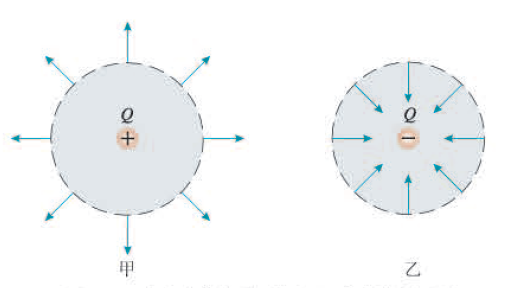
\includegraphics[width=0.5\textwidth]{point-charge-electric-field.png}
  \caption{点电荷的电场强度示意图}
  \label{fig:point-charge-electric-field}
\end{figure}

在距点电荷的距离相同的点构成的圆面上,电场强度的大小相同,方向与半径平行。

\subsection{电场线}

电场线是用于形象地表示电场的工具。它们是虚构的线条,表示电场的方向和强度。

电场线有以下性质

\begin{enumerate}
  \item 电场线的切线方向表示电场强度的方向。
  \item 电场线的密度表示电场强度的大小,电场线越密集,电场强度越大。
  \item 电场线从正电荷出发,指向负电荷。
  \item 电场线不能相交。
  \item 在均匀电场中,电场线平行且等距分布。
  \item 在非均匀电场中,电场线的密度变化表示电场强度的变化。
  \item 电场线的起点和终点分别是正电荷和负电荷,或者是无穷远处。
\end{enumerate}

\subsection{匀强电场}

\begin{definition}
  如果电场强度在空间的某一部分内的每一点都相等,则称该部分为\textbf{匀强电场(uniform electric field)}。在匀强电场中,电场线平行且等距分布。

  匀强电场的电场强度可以用以下公式表示:

  $$
  E = \frac{U}{d}
  $$

  其中 $U$ 是两点之间的电势差,$d$ 是两点之间的距离。
\end{definition}

\section{静电的防治与利用}

\subsection{静电平衡}

\begin{definition}
  将不带电的金属导体放到电场中,金属导体中的自由电子会在电场力的作用下发生定向移动,这个移动会生成一个与外界电场反向的电场,这两个电场叠加,最终导致金属导体内部的电场强度为零,这种状态称为\textbf{静电平衡(electrostatic equilibrium)}。
\end{definition}

静电平衡的性质\footnote{有几个应该高中是不要求的?}

\begin{enumerate}
  \item 在静电平衡状态下,导体内部的电场强度为零。
  \item 在静电平衡状态下,导体表面的电场强度垂直于导体表面。
  \item 在静电平衡状态下,导体表面的电荷分布与导体的形状有关,导体表面电荷密度在尖端处最大,在平坦处最小。
  \item 在静电平衡状态下,导体表面的电场线密度与导体表面的电荷密度成正比。
  \item 静电平衡状态下,导体内部没有净剩电荷。
\end{enumerate}

\subsection{尖端放电}

在静电平衡时,导体内部没有净剩电荷并且在尖端的电荷密度最大,当电荷密度达到一定程度时,导体表面的电场强度会足够大,以至于可以使空气中的分子电离,从而形成等离子体,这个现象称为\textbf{尖端放电(corona discharge)}。

在建筑物的顶端放置金属尖端,并且通过连接金属板的粗导线与大地相连接,形成避雷针,可以通过中和云层中的电荷,防止雷电直接击中建筑物。

\subsection{静电屏蔽}

当导体处于静电屏蔽状态时,导体内部的电场强度为零,这种现象称为\textbf{静电屏蔽(electrostatic shielding)}。静电屏蔽可以用来保护敏感电子设备免受外部电场的干扰。

\begin{figure}[htbp]
  \centering
  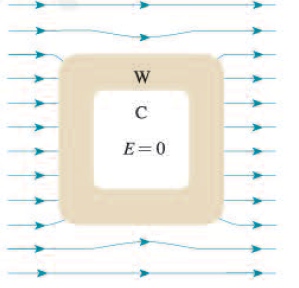
\includegraphics[width=0.3\textwidth]{electrostatic-shielding.png}
  \caption{静电屏蔽示意图}
  \label{fig:electrostatic-shielding}
\end{figure}

\subsection{静电吸附}

静电吸附是典型的利用静电现象。

\begin{itemize}
  \item \textbf{静电除尘}\\
    由带电的金属棒和板状的带电的收集器组成,金属棒带高压负电,收集板带正电。工作时金属棒附近的极强电场使得空气发生电离,正电荷离子吸附到金属棒上,负电荷向收集板移动,同时碰到灰尘胃里,使之带负电,向收集板移动,灰尘被收集板吸附。
  \item \textbf{静电喷漆}\\
    雾化器接有高压负电,使喷射出的油漆颗粒带负电;同时工件位于正极,使得油漆颗粒向工件移动,完成喷漆。
  \item \textbf{静电复印}\\
    静电复印机的核心是有机光导体鼓,无光照时是绝缘体,有光照时为导体。先对带有墨粉的鼓充电,然后对需要复印的部分进行光照,使得光照部分的鼓变为导体,墨粉被吸附到光照部分,不需要的部分则为绝缘体不带电落下。然后将鼓上的墨粉转移到纸上,最后加热使墨粉熔化,完成复印。
\end{itemize}

\chapter{静电场中的能量}

\section{电势能和电势}

在静电场中静电力做的功通过矢量的运算得到。设试探电荷的电荷量为 $q$,运动了 $\vec{r}$ 的距离,且电场强度为 $\vec{E}$,在这段距离上电场力做的功为:

$$
W = \vec{F} \cdot \vec{r} = q\vec{E} \cdot \vec{r}
$$

\begin{lemma}
  通过证明可以得出结论:电场为无旋场,即电场的旋度为零,电场力做功与路径无关。
  
  这样的力我们称为保守力,同样的力还有重力,引力等。
\end{lemma}

\begin{definition}
  在电场中电荷减少的能量被称为\textbf{电势能(electric potential energy)},用 $E_p$ 表示。
\end{definition}

我们通常使用 $W_{\text{AB}}$ 来表示从点 A 到点 B 的电场力做的功,设点 A 的电势能为 $E_p(A)$,点 B 的电势能为 $E_p(B)$,则有:

$$
W_{\text{AB}} = E_p(A) - E_p(B)
$$

\begin{itemize}
  \item 如果 $W_{\text{AB}} > 0$,则 $E_p(A) > E_p(B)$,表示静电力做正功,电势能减少
  \item 如果 $W_{\text{AB}} < 0$,则 $E_p(A) < E_p(B)$,表示静电力做负功,电势能增加
\end{itemize}

注意到静电力做功表示的是势能变化的情况,不能直接用来表示电势能的大小,要选择一个参考点来定义电势能的零点。通常选取无限远处作为电势 $0$ 点,或者选取地面为电势 $0$ 点。

电荷量翻倍时,电势能也翻倍,电势能和电荷量成正比,我们定义电势能和电荷量的比值为\textbf{电势(electric potential)},用 $\varphi$ 表示:

$$
\varphi = \frac{E_p}{q}
$$

电势的单位为伏特 (volt),符号为 V。1 伏特等于 1 焦耳/库伦。

电势在电场线上沿着电场线逐渐下降,并且与电势能相同,需要确定一个参考点来定义电势的零点。通常选取无限远处作为电势 $0$ 点。

\section{电势差}

在电场中,两点之间电势的差值为电势差,也叫电压(voltage),用 $U$ 表示

\begin{definition}
  两点之间的电势差定义为:

  $$
  U = \varphi(A) - \varphi(B) = \frac{E_p(A)}{q} - \frac{E_p(B)}{q}
  $$

  电势差的单位为伏特(volt),符号为 V。
\end{definition}


\end{document} 
